\section{Arduino DAQ full code}
\subsection{Arduino C++ Code}
\label{subsec:arduinoCppcode}
%%% ARDUINO CPP CODE
\begin{lstlisting}[style=cstyle, caption=C++ Code on Arduino, label=lst:arduinoCodeApp, language=C++]
    /*
    * Reads 4 analog inputs (0-5V) for recording_dur seconds
    * Streams data to PC while recording
    */
    // change to true to print debug messages on Serial Monitor
    // printing debug lines impacts transmission speed and messes csv
    //  do not leave on during measurements!
    bool debug = false;
  
    const int analogInputs[] = {A0, A1, A2, A3};
    
    
    // set up the global varialbes
    unsigned long start_time;
    const unsigned long recording_dur = 5000; // 25 seconds in milliseconds (ENSURE python code is greater than this)
    unsigned long last_sample_time = 0;
    const unsigned long min_samp_interval = 2; // Sample every 2ms (adjust for stability)
    bool recording = false;
    int sample_count = 0;
    
    void setup() {
      // serial communication at 115200 bps
      Serial.begin(115200);
      
      // Set pins as input
      for (int i = 0; i < 4; i++) {
        pinMode(analogInputs[i], INPUT);
      }
      
      // Optimize ADC for faster sampling
      // Set ADC prescaler to 16 (default is 128)
      //
      // Bit: 7:enable; 6: initiate a convertion 5: 
      //
      ADCSRA = (ADCSRA & 0xF8) | 0x04;
      
      // Wait for serial connection to establish
      delay(1000);
      
      // Send ready message
      Serial.println("ARDUINO_DAQ_READY");
    }
    
    void loop() {
      // Check if we received a command
      if (Serial.available() > 0) {
        String command = Serial.readStringUntil('\n');
        command.trim();
        
        if (command == "START") {
          if(debug) Serial.println("received START command");
  
          // Clear any remaining data in serial buffer
          while (Serial.available()) {
            Serial.read();
          }
          
          // Reset sample counter
          sample_count = 0;
          
          // Send header once
          Serial.println("Sample,Time(ms),A0(V),A1(V),A2(V),A3(V)");
          
          // Start recording
          recording = true;
          start_time = millis();
          last_sample_time = start_time;
          
          // Send confirmation
          Serial.println("RECORDING_STARTED");
        }
      }
      
      // If we're recording, collect and send data immediately
      if (recording) {
        if(debug) Serial.println("Recording!");
        unsigned long currentTime = millis();
        unsigned long elapsed_time = currentTime - start_time;
        
        // Check if we're still within the recording period
        if (elapsed_time <= recording_dur) {
          if(debug) Serial.println("elapsed time << duration");
          // Only sample at the specified interval
          if (currentTime - last_sample_time >= min_samp_interval) {
            last_sample_time = currentTime;
            
            // Increment sample counter
            sample_count++;
            
            // Start building the output string
            String data_string = String(sample_count) + "," + String(elapsed_time);
            
            // Multiplex through the four inputs sequentially
            for (int i = 0; i < 4; i++) {
              if(debug) Serial.println("reading input: " + String(i));
              int raw_value = analogRead(analogInputs[i]);
              float voltage = raw_value * (5.0 / 1023.0);
              data_string += "," + String(voltage, 3);
            }
            
            // Send the complete data string at once
            Serial.println(data_string);
          }
        }
        else {
          // End of recording
          recording = false;
          
          // Send notification that recording is complete
          Serial.println("RECORDING_COMPLETE");
          Serial.print("SAMPLES_COLLECTED:");
          Serial.println(sample_count);
          Serial.println("END_OF_DATA");
        }
      }
    }
  
\end{lstlisting}
%
%
%
%       ~~~~~~~~~~~~~~ PYTHON SERIAL RECEIVE APPENDIX ~~~~~~~~~~~                  %
%
%
\subsection{PC-side Python Serial Receive Script}
%%% Python Script
\begin{lstlisting}[style=pythonstyle, caption=Python Serial Receive Script, label=lst:pythonCodeApp, language=Python ]
    import serial
    import time
    import matplotlib.pyplot as plt
    import pandas as pd
    import os
    import numpy as np
    from scipy import signal
    
    def apply_lowpass_filter(data, fs):
        """Apply a 4-pole low-pass Butterworth filter with 5Hz cutoff"""
        cutoff_freq = 2.0
        filter_order = 4
        
        nyquist = 0.5 * fs
        normal_cutoff = cutoff_freq / nyquist
        # analog=False implies  bilinear Transformation
        b, a = signal.butter(filter_order, normal_cutoff, btype='low', analog=False)
        filtered_data = signal.filtfilt(b, a, data)
        
        return filtered_data
    
    # Load data from CSV, apply a 4-pole low-pass filter, and save the filtered data
    def filter_and_save_data(filename):
        
        # Read the CSV data to pandas DataFrame
        #  It knows what are the column names
        df = pd.read_csv(filename)
        
        # Clean the dataframe - convert all columns to numeric
        for col in df.columns:                  # v - write NaN where it can't convert to number (in teh data, not column names)
            df[col] = pd.to_numeric(df[col], errors='coerce')
    
        # remove rows with NaN (not a number)
        df = df.dropna()
        
        # Samples not at exact distance from each other
        # Calculate the sampling frequency (median of differences)
        # numpy.diff to get the difference between samples
        time_diffs = np.diff(df['Time(ms)'])
        # numpy.median to get the median
        median_time_diff = np.median(time_diffs)  # in milliseconds
        fs = 1000.0 / median_time_diff  # Convert to Hz
        
        # Filter each analog channel:
        # ID column head for each channel 
        analog_channels = ['A0(V)', 'A1(V)', 'A2(V)', 'A3(V)']
        # take each channel one at a time
        for channel in analog_channels:
            # if name maches a column name
            if channel in df.columns:
                # add a new column _filtered, and send the array containing all the raw values to 
                # have them filtered, and save them in the new _filtered column
                df[f"{channel}_filtered"] = apply_lowpass_filter(df[channel].values, fs)
        
        # Save the pandas Dataframe with filtered columns to a new CSV file
        filtered_filename = f"{os.path.splitext(filename)[0]}_filtered.csv"
        df.to_csv(filtered_filename, index=False)
        
        return filtered_filename
    
    #
    # Plot the DAQ data with original and filtered signals overlapped
    #
    def plot_data(filename):
        
        # Read the CSV data with pandas
        df = pd.read_csv(filename)
        
        # Initialize an empty list to store our analog channel names
        analog_channels = []
    
        # Look through all column names in the DataFrame
        for col in df.columns:
            # the column name starts with 'A'
            if col.startswith('A'):
                #  the column name ends with '(V)'
                if col.endswith('(V)'):
                    # the column name does NOT contain '_filtered'
                    if '_filtered' not in col:
                        # add this column name to our list
                        analog_channels.append(col)
        
        # Create color cycle for different channels
        colors = ['blue', 'green', 'red', 'purple']
        
        # Create a single plot with all channels overlapping
        plt.figure(figsize=(14, 8))
        
        # Plot original data (semi-transparent)
        for i, channel in enumerate(analog_channels):
            color = colors[i % len(colors)]
            plt.plot(df['Time(ms)'], df[channel], label=f'{channel} Original', 
                    linewidth=1.5, alpha=0.4, color=color, linestyle='-')
        
        # Plot filtered data (solid lines)
        for i, channel in enumerate(analog_channels):
            filtered_channel = f"{channel}_filtered"
            if filtered_channel in df.columns:
                color = colors[i % len(colors)]
                plt.plot(df['Time(ms)'], df[filtered_channel], label=f'{channel} Filtered', 
                        linewidth=2.5, color=color, linestyle='-')
        
        # Set the y-axis range from 0 to 5V
        plt.ylim(0, 5)
        
        # Add labels and title
        plt.xlabel('Time (ms)')
        plt.ylabel('Voltage (V)')
        plt.title('Arduino DAQ - 4-Channel Readings with 4-Pole 5Hz Low-Pass Filter')
        plt.legend()
        plt.grid(True)
            
        # Add data summary
        duration = df['Time(ms)'].max() - df['Time(ms)'].min()
        sample_count = len(df)
        sample_rate = sample_count/(duration/1000) if duration > 0 else 0
        
        info_text = f"Data summary:\n" \
                    f"Duration: {duration:.1f} ms\n" \
                    f"Samples: {sample_count}\n" \
                    f"Sample rate: {sample_rate:.1f} Hz\n" \
                    f"Filter: 4-pole Butterworth, 5Hz cutoff"
                    
        plt.figtext(0.02, 0.02, info_text, fontsize=10, 
                    bbox=dict(facecolor='white', alpha=0.8))
        
        # Save the plot
        plot_filename = f"{os.path.splitext(filename)[0]}_plot.png"
        plt.savefig(plot_filename, dpi=300, bbox_inches='tight')
        
        # Show the plot
        plt.tight_layout()
        plt.show()
    
    def main():
    
        # ASk if to plot or measure
        what_to_do = int(input("Record new measurement (1) or plot existing (2): "))
    
        # User selected to plot old csv
        if(what_to_do == 2):
            plot_data(input("Insert the name of the csv: "))
        
    
        # User selected to record new measurement
        elif(what_to_do == 1):
            # Use a default port (COM3 for Windows, modify as needed)
            default_port = "COM3"  # Change to match your system
            
            print(f"Using  port: {default_port}")
            
            # Configure serial port
            try:
                ser = serial.Serial(default_port, 115200, timeout=2)
                print("Connected to Arduino!")
            except serial.SerialException:
                print(f"Error: Could not open port {default_port}")
                print("Please modify the default_port variable in the script.")
                return
            
            time.sleep(2)  # Wait for Arduino to reset
            
            # Flush buffers
            ser.reset_input_buffer()
            ser.reset_output_buffer()
            
            # Wait for Arduino ready
            print("Waiting for Arduino to be ready...")
            ready = False
            timeout = time.time() + 10 # don't wait too long
            
            while not ready and time.time() < timeout:
                line = ser.readline().decode('utf-8', errors='ignore').strip()
                if line == "ARDUINO_DAQ_READY":
                    ready = True
                    print("Arduino is ready!")
            
            if not ready:
                print("Timed out waiting for Arduino. Make sure it's properly connected.")
                ser.close()
                return
            
            # Create a filename for this recording session
            filename = f"arduino_daq_data_{time.strftime('%Y%m%d_%H%M%S')}.csv"
            
            print(f"Starting data recording to {filename}...")
            print("Press Ctrl+C to stop if needed.")
            
            with open(filename, 'w', newline='') as file:
                # Send start command
                ser.write(b"START\n")
                
                recording = True
                data_lines = 0
                
                # Start time for timeout
                start_time = time.time()
                timeout_duration = 15  # seconds
                
                while recording and (time.time() - start_time) < timeout_duration:
                    if ser.in_waiting:
                        line = ser.readline().decode('utf-8', errors='ignore').strip()
                        
                        if "RECORDING_COMPLETE" in line:
                            recording = False
                            print("Recording complete!")
                        elif "END_OF_DATA" in line:
                            pass
                        elif line:
                            # Write the line to the file
                            file.write(line + '\n')
                            data_lines += 1
                            
                            # Show progress occasionally
                            if data_lines % 100 == 0:
                                print(f"Recorded {data_lines} data points...")
            
            # Close the serial port
            if ser.is_open:
                ser.close()
                print("Serial port closed.")
            
            print(f"Recorded {data_lines} lines of data.")
            
            # Process the data
            print("Applying filters to data...")
            filtered_filename = filter_and_save_data(filename)
            print(f"Filtered data saved to {filtered_filename}")
            
            print("Generating plot...")
            plot_data(filtered_filename)
            print("Done!")
            
        else:
            print("Wrong Choice. Goodbye!")
            exit()
    if __name__ == "__main__":
        try:
            main()
        except KeyboardInterrupt:
            print("\nProgram terminated by user.")
\end{lstlisting}

\section{Derivation of TIA Voltage Out}

% V out derivation
%
\begin{figure}[htbp] 
    \centering
    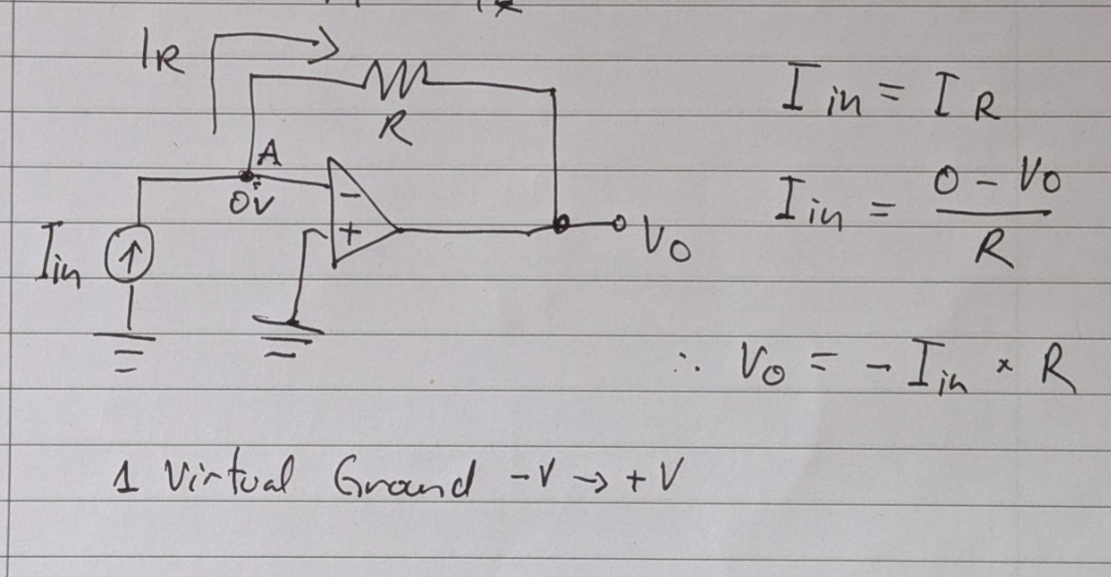
\includegraphics[width=0.8\textwidth]{figures/Appendix-DAQ/Vo_deriv.png}
    \caption{Solution Deriving TIA Vout}
    \label{fig:Vo_deriv}
  \end{figure}